\documentclass{article}
\usepackage{graphicx}
\usepackage{hyperref}
\usepackage{amsmath}
\usepackage{amssymb}

\title{CCE3015 - Assignment 1 – Problem Research and Planning}
\author{Graham Pellegrini}
\date{\today}

\begin{document}

\maketitle
\section{Question 1}
The Multi-level 3D Discrete Wavelet Transform (DWT) is an effective technique in signal processing, particularly useful for data compression and denoising applications. This transform decomposes a 3D dataset into sub-bands, capturing frequency components across multiple resolutions. Each decomposition level separates the data into approximation and detail coefficients, progressively breaking down the data into low and high frequency componenets.

\subsection{Problem Overview}
In this problem, we will be working with the CHOAS dataset \cite{CHAOSdata2019}, which contains large 3D medical images saved as slices in DICOM (.dcm) files. Given the dataset's size and format, these slices are first pre-processed in Python to convert them into a binary (.bin) file. The preprocessing pipeline involves reading DICOM files, transforming them into NumPy arrays, and saving the arrays as binary files. This binary format will allow for efficient loading and processing in the C++ implementation of the 3D DWT.

\begin{figure}[h]
    \centering
    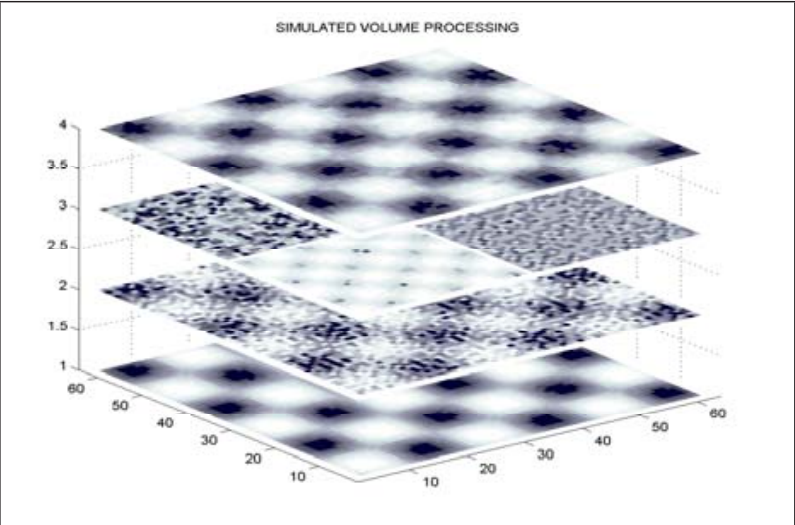
\includegraphics[width=0.8\textwidth]{assets/slices.png}
    \caption{3D Volume from 2D Slices \cite{Prochazka2011}}
    \label{fig1}
\end{figure}

In the preprocessing step, to achieve a 3D volume from 2D slices. The slices are stacked along the depth axis to form a 3D volume, as shown in \ref{fig1}above. This 3D volume is saved as a numpy array in Python and then converted to a binary file for input into the C++ program. Like this the dicom slices have been converted into their respective 3D image as a volume.\\

\subsection{Algorithm Overview}
To implement the 3D DWT in C++, we will follow these key steps:\\

\textbf{Input/Output Handling:} Two utility header files will be included, one to load the binary data into a 3D volume array and another to save the processed data back into a binary file. These functions will facilitate data handling between Python and C++.\\


\textbf{Wavelet Coefficients:} Daubechies wavelet filters will be used, taking from db1 till db4. These filter coefficients will directly be sampled from pywavelets, for comparison purposes.These coefficients will be hardcoded as vectors with seperation between low-pass and high-pass filters. The filters will be applied to the 3D data in the convolution step. Having the low filters and high filters seperated will allow for easy implementation of the convolution step. The low emphasise the approximation coefficients and the high emphasise the detail coefficients of the signal.\\

\textbf{Discrete Wavelet Transform (DWT):} 
\begin{figure}
    \centering
    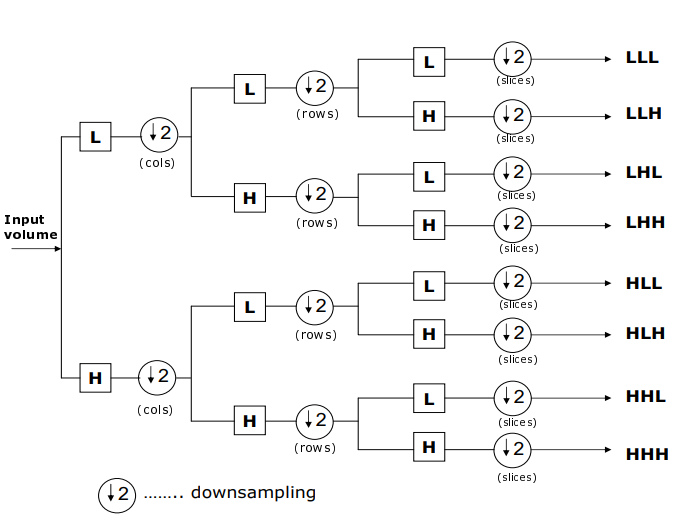
\includegraphics[width=0.8\textwidth]{assets/dwt.png}
    \caption{Discrete Wavelet Transform \cite{Prochazka2011}}
    \label{fig2}
\end{figure}

The pipeline shown in \ref{fig2} shows how the 3D volume can be spilt into 8 subbands. However first a function to perform the 1D DWT on a signal will be defined. This function will take the signal and convolve it with the low-pass and high-pass filters. The two seperated convolved otuputs will then be downsampled by selecting every second value. The downsampling technique is there as a way to reduce the data size by half along each axis as well as a data redundancy reduction technique.\\

This 1D DWT function will then be called three times in the 3D DWT function, as it will be applied to each axis of the 3D volume. The 3D DWT function will take the 3D volume and apply the 1D DWT function to each axis. To keep convention the dwt is first applied to the column axis and the respective L and H subbands will be stored back to the original volume. Then the dwt is applied to the row axis and now we get the LL LH HL HH subbands. Finally the dwt is applied to the depth axis and we get the 8 subbands (LLL LLH LHL LHH HLL HLH HHL HHH). So the order 3D DWT fucntion will include 3 nested for loops to apply the respective column-wise, row-wise and depth-wise DWT.\\

\begin{figure}
    \centering
    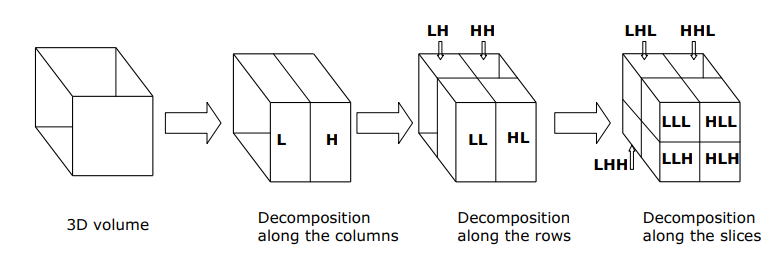
\includegraphics[width=0.8\textwidth]{assets/subbands.png}
    \caption{3D DWT Subbands \cite{Prochazka2011}}
    \label{fig3}
\end{figure}

The importance of always saving back the L and H subbands to the original volume is so we utalise memory efficiently, especially since we are working with 3d vectors of a large dataset.

\textbf{Multi-level Transform:} Our implementation aims at achieving Multi-level 3D DWT. This means we can take the approximation coefficients (LLL) from the first level and apply the 3D DWT again to get the approximation coefficients of the next level. This process can be repeated for as many levels as desired. However, it is important to note that while there is no theoretical limit to the number of levels, practical constraints are imposed by the image dimensions. In our case since the slices have dimensions of 78x256x256, a 4-level decomposition results in dimensions of 10x64x64, beyond which further decomposition would degrade image quality excessively.\\

A multi-level function will be defined that will call the 3D DWT function for the number of levels specified. If the level is not the final one then the volume dimensions will be halved along each axis, taking the approximation coefficients (LLL) and applying the 3D DWT function to them. In this process the higher level detail coefficients are discarded but they are not needed.\\
 
To be able to handle odd dimensions, either the dimention division must handle odd numbers or the volume must be padded with zeros to make the dimensions even.\\

\subsection{Evaluation and Testing}
To evaluate the implementation, we will have a post-processing step in Python. The saved output binary file will be loaded back into Python, and the 3D volume will be reconstructed from the subbands. This reconstructed coefficients will be compared to those achieved on the same volume with pywavelets. The comparison will be both visual and quantitative, using metrics like Mean Squared Error (MSE) and Eucaledian Distance. Although, we will be using the same coefficients as pywavelets, there might still be some differences in implementation. Such as the convolution, downsampling techniques and padding techniques. So the graphical comparison will be the main objective and then the statistical comparison will be a bonus to see how close the implementation is to the pywavelets implementation.\\

\section{Question 2}
To plan an efficient parallel implementation of the 3D Discrete Wavelet Transform (DWT) using CUDA, we analyze the operations that can be vectorized and optimized to exploit parallelism across the GPU's architecture. 

\subsection{Identifying Parallel Operations}
In the DWT process, each dimension of the 3D volume undergoes convolution with wavelet filters. This can be done in parallel for each row, column, and depth slice independently. By assigning each thread to handle a single 1D operation, such as convolution in the depth or row dimension, we maximize parallel processing across GPU threads. 

\subsection{Required Synchronization Points}
Synchronization points are necessary when switching between different dimensions of the 3D array (e.g., moving from row operations to column operations). This ensures data consistency before threads process the next dimension. CUDA’s `__syncthreads()` can be used here to synchronize threads within each block.

\subsection{Planning Sequence of Functions and Mapping to CUDA Architecture}
1. **Data Loading**: First, data is loaded onto the GPU's global memory. Each dimension is then processed independently in parallel.
   
2. **1D DWT on Rows and Columns**: Each 1D DWT operation is assigned to CUDA threads in a grid-block configuration. Using CUDA vectors for 3D volumes will reduce clock cycles due to memory coalescing.
   
3. **Loop Unrolling**: Unrolling inner loops of the convolution operations reduces the overhead associated with branch predictions, thus enhancing efficiency. For fixed wavelet filter sizes, this technique is particularly effective as it minimizes loop iteration overheads.

4. **Block and Thread Selection**: Choosing the number of blocks and threads requires careful consideration to avoid underutilizing or overfitting to the GPU’s capabilities. Optimal values are initially estimated based on input dimensions and then fine-tuned through testing to balance computational load. However, tuning may risk overfitting to specific datasets, reducing performance on varied data.

5. **Multi-Level Processing and Halving Dimensions**: At each level, the array size is halved, further reducing the workload for subsequent levels. After each level, threads synchronize to ensure data integrity before proceeding.

This design aligns well with the CUDA architecture by mapping independent tasks to separate threads, utilizing shared memory for intermediate results, and applying loop unrolling for efficiency in repetitive convolution tasks.

--okay so maybe mention points on vectorizing since we have a 3D volume if we perform them as CUDA vectors they will computationally take take less clock cycles. Mention how you would loop unroll ect...
--Mention that the amount of blocks /threads would be chosen and some parameters are trivial and must be tested manually but could run into the problem of overfitting.
\end{document}
